%!TEX root = ../Report.tex

In this chapter, we present specific implementation details of the project, providing relevant code highlights,and cover the problems that occurred and how they were solved.

We start with the implementation of a basic skeleton, then we cover adding plasticity, and contention aware scheduling. Finally, we cover the applications developed to evaluate the project.

C++ was chosen as a basis, as it is fast, and provides language constructs such as templates and overloading. Another, personal, reason is that I wished to learn something new, as I had not used C++ before. 

The parallel backend that the system is based upon is Pthreads due to its wide availability, and the level of fine control. It allows us to tune all parameters of the program and implement functions which are not possible with other solutions, e.g. detailed metric analysis. 



\section{Skeleton Foundation}
\label{section:implementation_skeleton_foundation}

The first skeleton we will implement is the map-array skeleton, as described in section \ref{section:design_skeleton_foundation}. It is reasonably straight forward to create a sequential skeleton, using C++ templates to create a templated function which takes another function amongst other things as its arguments. This will be our skeleton. The interface of our skeleton is given in figure \ref{fig:implementation_map_array_interface}, and a usage example in figure \ref{fig:implementation_map_array_usage_example}.



\begin{figure}
	\begin{lstlisting}

	template <typename in1, typename in2, typename out>
	void map_array(deque<in1>& input1, 
				   	deque<in2>& input2, 
				   	out (*user_function) (in1, deque<in2>), 
				   	deque<out>& output, 
				   	string output_filename = "", 
				   	parameters params = parameters())

	\end{lstlisting}

	\caption{Interface of our map\_array skeleton. The first four variables are the two input arrays, the function to apply, and the output array respectively. The output\_filename variable is the filename to record the metrics output in, and params sets up the initial parameters we will use. These last two are optional.}
	\label{fig:implementation_map_array_interface}
\end{figure}



\begin{figure}
	\begin{lstlisting}
	int user_function(int in1, deque<int> in2) {
		return in1 + in2[in1];
	}

	int main() {
		// Inputs.
		deque<int> input1(ARRAY_SIZE);
		deque<int> input2(ARRAY_SIZE_2);

		// Put data in inputs.

		// Output.
		deque<int> output(ARRAY_SIZE);

		// Start mapArray.
		map_array(input1, input2, user_function, output);

		// Record output.
	}
	\end{lstlisting}

	\caption{A usage example of map\_array, here we apply our user\_function to each element of input1. The size of our two input arrays need not match, but the size of the input1 and output arrays must.}
	\label{fig:implementation_map_array_usage_example}
\end{figure}



\begin{minipage}{\textwidth}

Parallelizing this presents two problems, namely:

\begin{itemize}
	\item How to divide tasks amongst threads (in map array, a task is one application of the user function to an element of the input array)
	\item How many threads should be used
\end{itemize}

\end{minipage}
 
In a basic skeleton, both of these parameters must be specified beforehand and will not change at runtime. The ability to vary them would provide the different implementations necessary for the plasticity portion of this project.

To implement multiple schedules, we use a bag of tasks object. A bag of tasks is a collection of independent, usually similar tasks which are to be executed. It is a model which is usually combined with some form of parallelism.

Each thread will be given the location of the same bag, and will retrieve a specified number of tasks at a time from the bag. Since each schedule essentially consists of retrieving a different number tasks at a time, we can use this to implement the basic schedules (Static, Dynamic Chunks, Dynamic Individual). More complex schedules can easily be added in the future, as they can reuse the same framework, and simply adjust how many tasks each thread retrieves at one time.

The bag also provides the main source of inter-thread communication using shared memory, and contains various semaphores for controlling the threads. This will be expanded upon in sections \ref{section:implementation_adding_plasticity} and \ref{section:implementation_contention_aware_scheduling}.

This bag of tasks object also gives us the basis for further extensions, such as using multiple bags, adding task stealing, or adding tasks to the bag during computation.

Providing a variable number of worker threads is simple now that we have the bag of tasks, all we need to do is to adjust our initial calculations when calculating how many tasks each thread should receive according to the schedule. These worker threads will be spawned by the original thread, the ``main'' thread. It blocks until the computation is complete, it will then join with each of the worker threads.

Figure \ref{fig:implementation_create_threads} shows how we create our worker thread using Pthreads, and figure \ref{fig:implementation_join_threads} hows how we later join with them.



\begin{figure}
	\begin{lstlisting}
	template <typename in1, typename in2, typename out>
	void map_array(. . .) {
	  . . .
	  // Calculate info for data partitioning.
	  deque<thread_data<in1, in2, out>> thread_data_deque = calc_thread_data(bot.numTasksRemaining(), bot, params);
  
	  // Variables for creating and managing threads.
	  deque<pthread_t> threads(params.thread_pinnings.size());
  
	  // Create all our needed threads.
	  for (uint32_t i = 0; i < params.thread_pinnings.size(); i++) {
	    int rc = pthread_create(&threads.at(i), NULL, mapArrayThread<in1, in2, out>, (void *) &thread_data_deque.at(i));
  
	    // Create thread name.
	    char thread_name[16];
	    sprintf(thread_name, "MA Thread %u", i);
  
	    // Set thread name.
	    pthread_setname_np(threads.at(i), thread_name);
  
	    if (rc) {
	      // If we couldn't create a new thread, throw an error and exit.
	      print("[Main] ERROR; return code from pthread_create() is ", rc, "\n");
	      exit(-1);
	    }
	  }
	  . . .
	}
	\end{lstlisting}

	\caption{The parallel portion of our map\_array skeleton. This figure shows how we use Pthreads to create our worker threads, providing each with access to its own thread data object.}
	\label{fig:implementation_create_threads}
\end{figure}



\begin{figure}
	\begin{lstlisting}
	// Joins with given number of threads. 
	void join_with_threads(std::deque<pthread_t> threads, uint32_t num_threads_to_join) {
	  int inital_threads_max_index = threads.size() - 1;

	  for (uint32_t i = 0; i < num_threads_to_join; i++) {
	    // Join with thread
	    int rc = pthread_join(threads.back(), NULL);

	    // Update thread tracking variables.
	    threads.pop_back();

	    if (rc) {
	      // If we couldn't join with the thread, throw an error and exit.
	      print("[Main] ERROR; return code from pthread_join() is ", rc, "\n");
	      exit(-1);
	    }
	  }
	}
	\end{lstlisting}

	\caption{Function which joins with the specified number of threads. Starts with the last thread to be created, so that if we wish to terminate threads, the threads which remain executing preserve their logical ordering.}
	\label{fig:implementation_join_threads}
\end{figure}



\section{Adding Plasticity}
\label{section:implementation_adding_plasticity}

We already have a type of compile time plasticity in our system, in that we can choose some parameters of the skeleton before compilation. We can choose the number of worker threads and the schedule used. The other main aspect we would like to control is what CPU core each thread executes on. This is called processor affinity or thread pinning. This was added to the skeleton by adding control variables to the bag of tasks, which control the CPU affinity of each thread. Each thread then simply sets its affinity to the intended CPU, using the function given in figure \ref{fig:implementation_thread_pinning}.

To add runtime plasticity, we need to be able to change the implementation of the skeleton on the fly. The most straightforward method of achieving this is to stop all computation, terminate worker threads, update the parameters, and resume computation. In a basic skeleton, (as described at the end of section \ref{section:implementation_skeleton_foundation},) the main thread would block until the computation is complete, and then would join with each of the worker threads. We change this so that, instead of blocking, it monitors the computation and can instruct the threads to terminate at any point (using the afore mentioned bag of tasks described in section \ref{section:implementation_skeleton_foundation} for communication. This functionality is shown in figure \ref{fig:implementation_bot_comms}). An overview of the code used to implement the process can be seen in figure \ref{fig:implementation_main_thread_bot_comms}.

When this switching is done and what the new parameters should be is another matter. A future system would calculate these things taking into account the current state of the system, but for our preliminary investigation, we manually produce them in a synthetic environment, and communicate them to the main thread using the controller application, as described in section \ref{section:implementation_contention_aware_scheduling}.

An obvious optimization of this system would be to modify the implementation without the need to terminate threads. This graceful switching of the implementation is left for future work, as this optimization is very complex, and would likely result in a marginal speedup proportional to the number of times we wish to change the implementation. We do not plan on switching implementations excessively, and any delay added could be overcome in testing by increasing the input size, and this project is only investigating if this approach to parallel programming is promising.

Another optimization would involve modifying the static schedule. In our implementation, worker threads only check if they should terminate when they contact the bag for more tasks. Since the static schedule means they only contact the bag at the start of the computation, once they have started, they cannot be interrupted. To optimize this, and make a "plastic" static schedule, we could change the communication method so that worker threads can be interrupted. For our later experiments, we hard-coded the switch, and the creation of a truly plastic static schedule has been left for future work.



\begin{figure}
	\begin{lstlisting}
	template <typename in1, typename in2, typename out>
	void map_array(. . .) {
	  . . .
	  while (bot.empty == false) {
  
	    // Get message from controller.
  
        // Terminating threads.
        bot.thread_control.assign(params.thread_pinnings.size(), Terminate);
  
        // Joining with threads.
        join_with_threads(threads, params.thread_pinnings.size());
  
        // Update parameters.
  
        // Restart map_array.
  	    
	  }
	  . . .
	}
	\end{lstlisting}

	\caption{An example of how the main thread handles a switch in the implementation.}
	\label{fig:implementation_main_thread_bot_comms}
\end{figure}



\begin{figure}
	\begin{lstlisting}
	// Thread control enum. Threads either run (execute), change strategies (update), or stop (terminate).
	enum Thread_Control {Execute, Update, Terminate};

	template <class in1, class in2, class out>
	class BagOfTasks {
	  public:
	    // Variables to control if threads terminate.
	    deque<Thread_Control> thread_control;

	    // Check for if bag is empty.
	    bool empty = false;
	    . . .

	    // Returns specified number of tasks or less. 
	    tasks<in1, in2, out> getTasks(uint32_t num) {
	      // Get mutex. 
	      lock_guard<mutex> lock(m);
		  . . .

		  // Calculate number of tasks to return.
		  . . .

		  if (num_tasks == 0) {
		    empty = true;
	      }
		  . . .
		}
	};
	\end{lstlisting}

	\caption{The inter-thread communication sections of the bag of tasks object. ``thread\_control'' provides a control variable for each thread, which the thread reads and reacts to. The ``empty'' boolean is updated when the getTasks method is run, and is read periodically by the main thread to check if we have completed the computation.}
	\label{fig:implementation_bot_comms}
\end{figure}



\begin{figure}
	\begin{lstlisting}
	// Sticks current thread to given CPU core.
	int stick_this_thread_to_cpu(uint32_t core_id) {
	   uint32_t num_cores = sysconf(_SC_NPROCESSORS_ONLN);

	   // Check for valid core_id.
	   if (core_id >= num_cores) {
	      return EINVAL;
	    }

	   cpu_set_t cpuset;
	   CPU_ZERO(&cpuset);
	   CPU_SET(core_id, &cpuset);

	   pthread_t current_thread = pthread_self();    

	   return pthread_setaffinity_np(current_thread, sizeof(cpu_set_t), &cpuset);
	}
	\end{lstlisting}

	\caption{Function for sticking the current thread to a particular CPU core. Enables thread pinning plasticity.}
	\label{fig:implementation_thread_pinning}
\end{figure}



\section{Contention Aware Scheduling}
\label{section:implementation_contention_aware_scheduling}

As detailed in section \ref{subsection:design_contention_aware_scheduling} of the design chapter, we will use a separate controller application to co-ordinate and control all programs using our library. This simplifies the implementation significantly, as it gives us a single point of contact, and a single place to calculate an optimal configuration for each program. To achieve this, we need our separate controller application, and two main additions to our system:

\begin{itemize}
	\item Inter-process communication (between the controller and each program)
	\item Separate communication/control thread for each program
\end{itemize}

We use the ZeroMQ library to provide inter-process communication due to its speed, although it could be replaced with another method. It uses tcp sockets, and serves to simplify inter-process communication. Currently I have made simple use of ZeroMQ for now, and may optimize it in the future. For inter-thread communication (between a main thread and worker threads), we use shared memory, again for speed.

In order to communicate with the controller while a program is using our library, we utilize the main thread, which will manage the worker threads, switch implementations when instructed, and will clean up after we have finished our computation. The main thread communicates with the controller, registering with it when we start and de-registering once complete. During computation, it listens to messages from the controller using non-blocking communication. This allows us to also check if we are finished processing the computation. For the initial registration and de-registration, we use blocking communication, as these messages are vital to the system. This system is illustrated at a high level in figure \ref{fig:controller_flowchart}, which expands upon figure \ref{fig:communication_structure}, showing implementation details. Figure \ref{fig:implementation_controller_comms} provides an example of the code used to perform this, and shows the use of the ZeroMQ library.



\begin{figure}
	\centering
	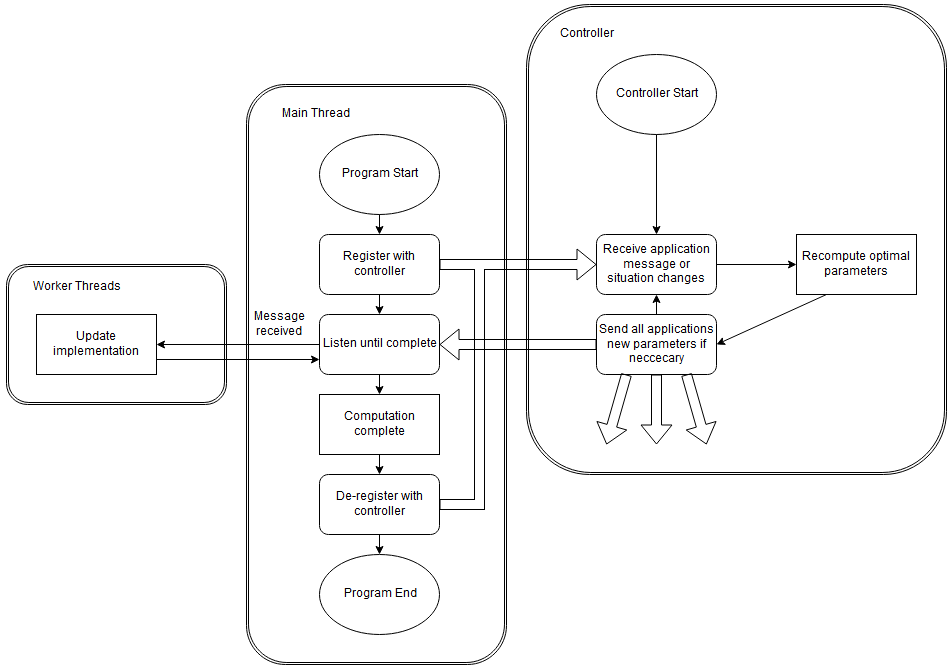
\includegraphics[width=1.1\textwidth]{graphics/controller_communication_flowchart.png}
	\caption{Communication model for communications between applications and the controller. Thin lines represent program flow, thick lines represent inter-process messages.}
	\label{fig:controller_flowchart}
\end{figure}



\begin{figure}
	\begin{lstlisting}
	template <typename in1, typename in2, typename out>
	void map_array(. . .) {
	  . . .
	  // Get our PID to send to the controller.
	  uint32_t pid = pthread_self();

	  // Prepare our context and socket
	  context_t context(1);
	  socket_t  socket(context, ZMQ_PAIR);
	  socket.connect("tcp://localhost:5555");

	  print("\n[Main] Registering with controller...\n\n");
	        
	  // Create registration message.
	  struct message rgstr;
	  rgstr.header                   = APP_REG;
	  rgstr.pid                      = pid;
	  rgstr.settings.schedule        = params.schedule;

	  fill_n(rgstr.settings.thread_pinnings, MAX_NUM_THREADS, -1);
	  copy(params.thread_pinnings.begin(), params.thread_pinnings.end(), rgstr.settings.thread_pinnings);

	  // Send registration message.
	  m_send(socket, rgstr);

	  while (bot.empty == false) {
	    usleep(1);

	    // Get message from controller. (Use a non-blocking receive so we can still check if bot.empty == true)
	    struct message msg = m_no_block_recv(socket);

	    if (msg.header == APP_UPDATE) {
	      print("\n[Main] Received new parameters from controller!\n\n");

	      // Update parameters.
	    }
	  }

	  // Create termination message.
	  struct message term;
	  term.header = APP_TERM;
	  term.pid = pid;

	  // Send termination message.
	  m_send(socket, term);

	  socket.close();
	\end{lstlisting}

	\caption{An example of how the main thread implements a change to the parameters received from the controller. Demonstrates the usage of the ZeroMQ library to provide inter-process communication with the controller.}
	\label{fig:implementation_controller_comms}
\end{figure}



\section{Testing Programs}

To evaluate our library, we need programs to run and test the library under differing conditions, and we need programs to represent the competing approaches to parallel programming. 

The main map-array test application is a tool which can read experimental parameters from a configuration file, and then run each experiment in sequence, recording various metrics for later analysis. This provides a convenient framework for carrying out experiments, and easily enables us to queue up a set of same. This is important from a time efficiency point of view because such experiments can take hours.

For meaningful analysis, we need to synthesize a workload. One which we can scale, so we can test different sized tasks and varying task distributions. To do this we use the Collatz function to generate a CPU intensive workload. A constant starting number is used, and the sequence is repeated multiple times, to scale accordingly.

The comparison programs consist of a purely sequential implementation, and an OpenMP implementation. These were chosen because the former represents an implementation a traditional sequential programmer would use, and OpenMP because it is a popular method of parallelizing code, with a focus on performance and a simple interface. They are set up such that they can use the same synthetic workload we use for testing our library.

The final tool we constructed for evaluation is a set of python programs which create graphs from the generated data.



\section{Utility Code}

This project required complex code to achieve its goals. In this section, we present other extracts of code, demonstrating its complexity. 

Basic functions must be reworked when we introduce parallelism to a program, let alone plasticity and contention aware scheduling. Figure \ref{fig:implementation_thread_safe_print} demonstrates a thread safe method for printing, by enforcing a mutex to be obtained before printing.

Figure \ref{fig:implementation_execute_external_program} shows how multiple programs were launched for testing. This was used in the testing framework, in experiment 5 for launching the additional programs at regular intervals.

\begin{figure}
	\begin{lstlisting}
	// .hpp file:

	// Print function entry point. Defaults to the cout output stream.
	template <class ...Args>
	std::ostream& print(const Args& ...args) {
	    std::lock_guard<std::mutex> _(get_cout_mutex());
	    return print(std::cout, args...);
	}

	// Retrieve mutex. This must be done using this non-templated function, so that we have one mutex instance across all instantiations of the templated functions.
	std::mutex& get_cout_mutex();

	// Case when given an output stream.
	template <class ...Args>
	std::ostream& print(std::ostream& outS, const Args& ...args) {
	    return print_rec(outS, args...);
	}

	// Recursively prints arguments.
	template <class A0, class ...Args>
	std::ostream& print_rec(std::ostream& outS, const A0& a0, const Args& ...args) {
	    outS << a0;
	    return print_rec(outS, args...);
	}

	// With nothing to add, just return the stream. 
	std::ostream& print_rec(std::ostream& outS);

	// .cpp file:

	// With nothing to add to the output stream, just return the stream.
	std::ostream& print_rec(std::ostream& outS) {
	    return outS;
	}

	// Retrieve mutex.
	std::mutex& get_cout_mutex() {
		// Static, so that we have one mutex instance across all instantiations of the templated functions.
	    static std::mutex m;
	    return m;
	}
	\end{lstlisting}

	\caption{A thread safe print function. Prints a variable type of and a variable number of arguments to an output stream. Implementation is split accross .hpp and .cpp files, as the need for templates requires that certain functions must be defined in the header, so the compiler can see them during linking.}
	\label{fig:implementation_thread_safe_print}
\end{figure}



\begin{figure}
	\begin{lstlisting}
	// Example usage: 

	const char *args[64] = {"../bin/program_2_map_array_test" , "../build/configs/config7.ini" , NULL};
    int out = exec_prog(args);

	static int exec_prog(const char **args) {
	    pid_t pid;
	    int   status, timeout;

	    if ((pid = fork()) == 0) {
	        if (execve(args[0], (char **)args , NULL) == -1) {
	            perror("fork() failed [%m]");

	            return -1;
	        }
	    }


	    timeout = 1000;

	    while (waitpid(pid , &status , WNOHANG) == 0) {
	            if (--timeout < 0) {
	                    perror("timeout");

	                    return -1;
	            }

	            sleep(1);
	    }

	    printf("%s WEXITSTATUS %d WIFEXITED %d [status %d]\n\n", args[0], WEXITSTATUS(status), WIFEXITED(status), status);

	    if (WIFEXITED(status) != 1 || WEXITSTATUS(status) != 0) {
	            perror("%s failed, halt system");

	            return -1;
	    }

	    return 0;
	}
	\end{lstlisting}

	\caption{A function for executing an external program, used in the setup for experiment 5.}
	\label{fig:implementation_execute_external_program}
\end{figure}